% Ubah kalimat sesuai dengan judul dari bab ini
\chapter{PEMBAHASAN}

% Ubah konten-konten berikut sesuai dengan yang ingin diisi pada bab ini

\section{Latar Belakang Pembuatan Aplikasi}

Batik merupakan sebuah warisan budaya bangsa Indonesia yang harus dilestarikan.
Terlebih lagi, pada tanggal 2 Oktober 2009, batik terdaftar sebagai warisan budaya dunia oleh UNESCO.
Berdasarkan data dari budaya-indonesia.org, terdapat 5849 variasi/motif batik di Indonesia \cite{jumlahBatik}.
Dengan jumlah variasi yang terhitung tidak sedikit tentu saja bukan hal yang mudah untuk orang awam untuk mengenali tiap variasi dari motif batik yang ada di Indonesia yang lalu berdampak pada keadaan dimana batik kurang terlalu diperhatikan atau dikenal.

Aplikasi Identifikasi Motif Batik yang kami beri nama \textbf{The Batik} yang kami rencanakan untuk diikutsertakan dalam program \textit{Capstone Project} ini merupakan aplikasi android yang dapat mengidentifikasi motif batik yang dikirim lewat aplikasi ini.
Maksud dari pengembangan proyek ini adalah untuk dapat membantu orang mengenali batik yang sedang mereka lihat secara langsung dan cepat melalui bantuan dari aplikasi yang ada di \textit{smartphone} pengguna.
Dengan begitu tidak memerlukan seorang ahli batik dalam mengetahui atau mengenal batik yang sedang dilihat.
Aplikasi ini juga dilengkapi dengan informasi mendetail untuk dari batik yang sudah dipindai seperti asal–usul dan sejarahnya.
Selain itu aplikasi ini juga dilengkapi daftar toko yang menjual batik yang sudah dipindai sehingga secara tidak langsung dapat membantu usaha batik lokal.

\section{Pembuatan Perangkat Lunak}

  \subsection{Pengembangan Aplikasi Android}

  \begin{figure}[hpt!]

    \centering
    \begin{subfigure}[b]{0.3\textwidth}
      
      \centering
      
      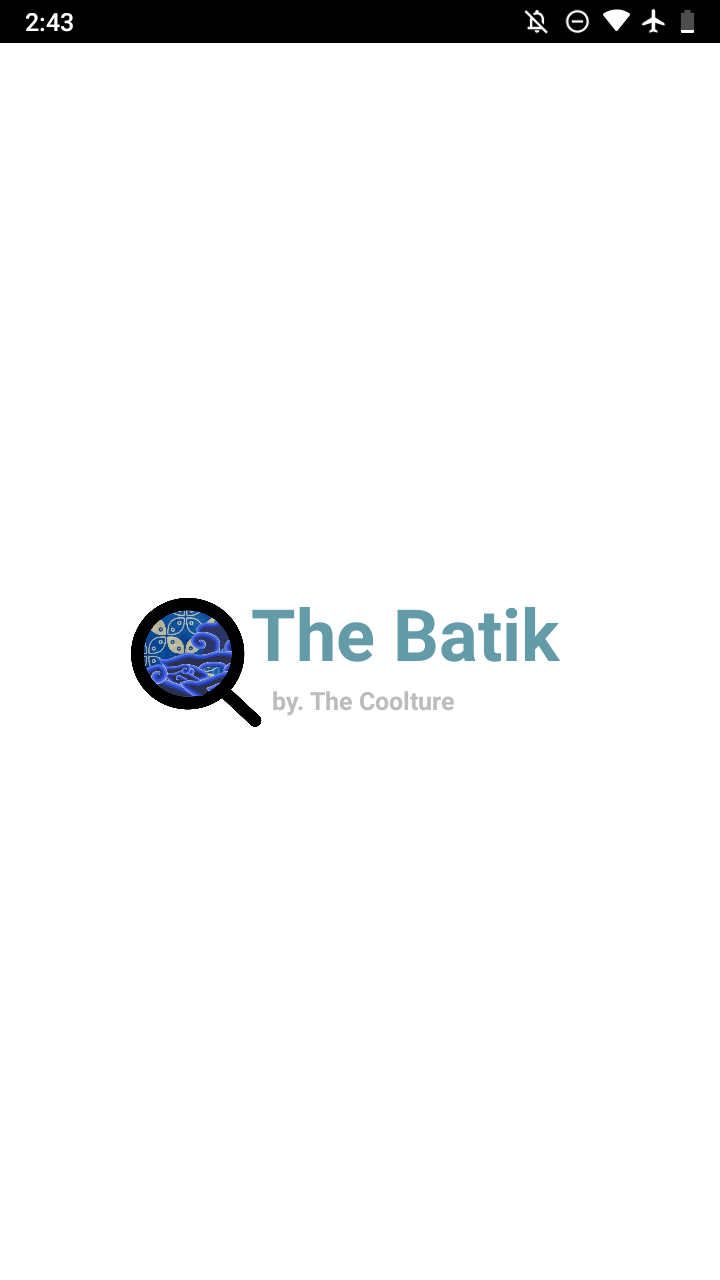
\includegraphics[width=\textwidth]{gambar/satu.png}
      
      \caption{Halaman Depan}
      
      \label{fig:satu}

    \end{subfigure}
    \hfill
    \begin{subfigure}[b]{0.3\textwidth}
      
      \centering
      
      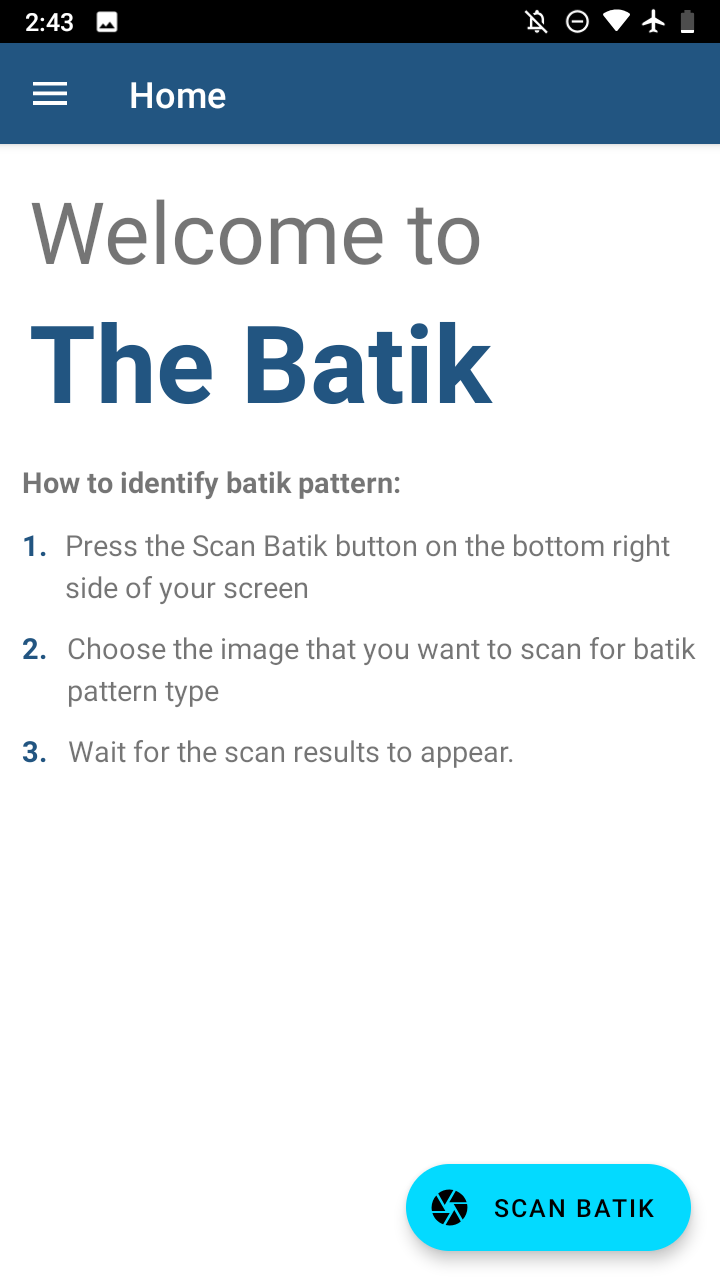
\includegraphics[width=\textwidth]{gambar/dua.png}
      
      \caption{Pemindai Batik}
      
      \label{fig:dua}
    \end{subfigure}
    \hfill
    \begin{subfigure}[b]{0.3\textwidth}
      
      \centering
      
      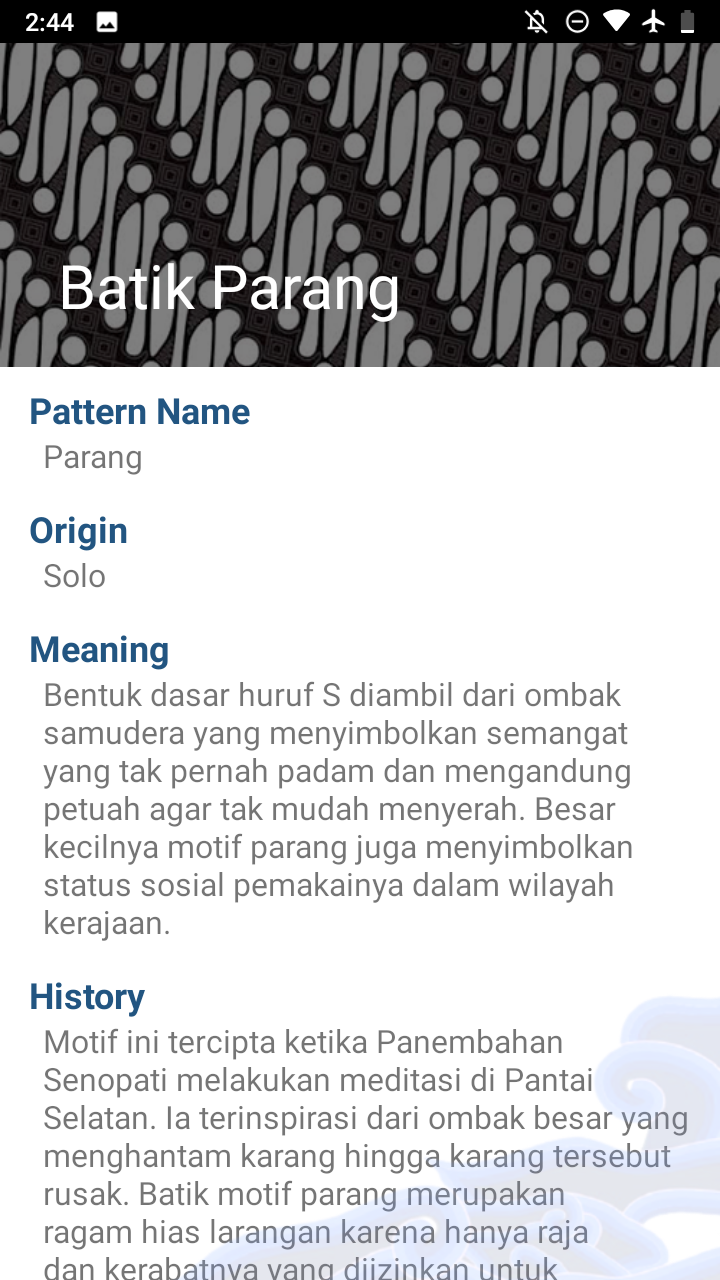
\includegraphics[width=\textwidth]{gambar/tiga.png}
      
      \caption{Deskripsi Batik}
      
      \label{fig:tiga}
    \end{subfigure}
    \\
    \begin{subfigure}[b]{0.3\textwidth}
      
      \centering
      
      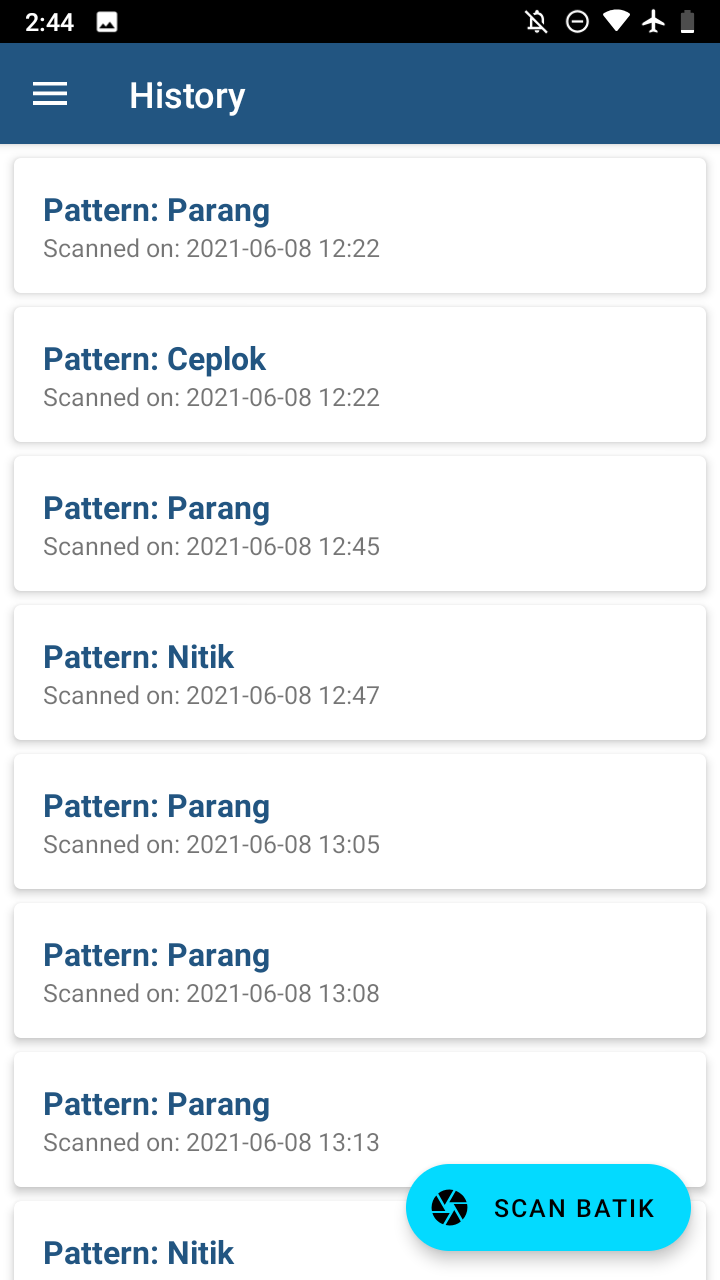
\includegraphics[width=\textwidth]{gambar/empat.png}
      
      \caption{Deskripsi Batik}
      
      \label{fig:empat}
    \end{subfigure}
    \hfill
    \begin{subfigure}[b]{0.3\textwidth}
      
      \centering
      
      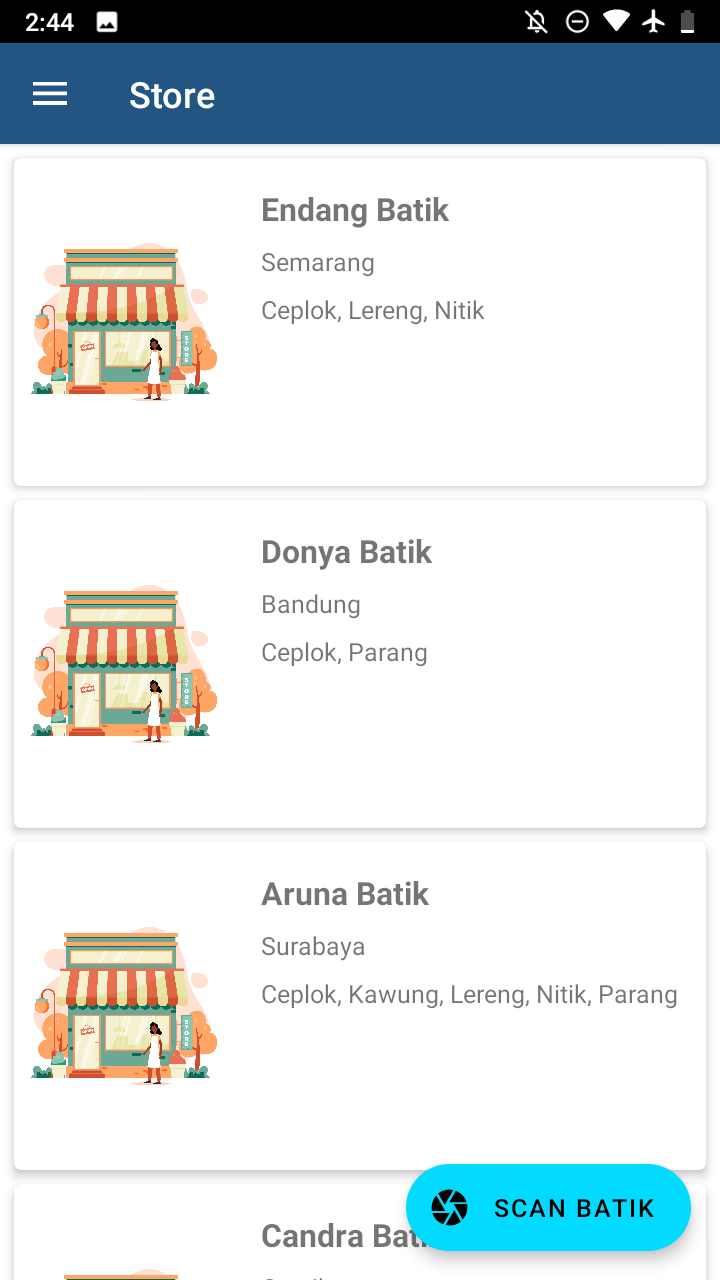
\includegraphics[width=\textwidth]{gambar/lima.png}
      
      \caption{Toko Batik}
      
      \label{fig:lima}
    \end{subfigure}
      
    \caption{Tampilan Aplikasi Android}
    \label{fig:android}
  
  \end{figure}

  Penggembangan aplikasi Android yang menjadi garis depan antara pengguna dan proyek ini dikembangan dengan Android Studio yang menggunakan bahasa pemrograman Kotlin.
  Pengembangan aplikasi android ini sendiri tidak dilakukan oleh penulis dari laporan ini melainkan oleh peserta Google Bangkit lainnya yang berasal dari kurikulum \textit{Mobile Development}.

  \subsection{Pembuatan Model \textit{Machine Learning}}
  
  \begin{figure}[htp!] \centering
    % Nama dari file gambar yang diinputkan
    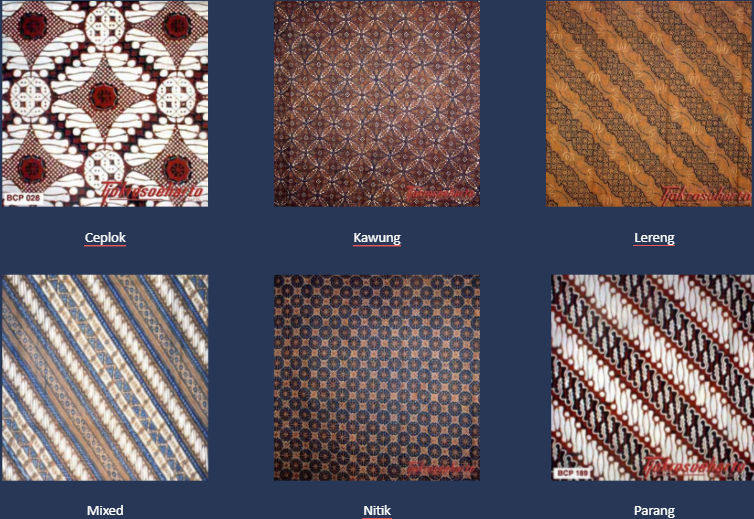
\includegraphics[scale=0.3]{gambar/batik.png}
    % Keterangan gambar yang diinputkan
    \caption{Pola Batik \cite{gultom2018batik}}
    % Label referensi dari gambar yang diinputkan
    \label{fig:polaBatik}
  \end{figure}
  
  Untuk dataset \cite{gultom2018batik}, kami menggunakan dataset yang berisi 6 pola batik yang berbeda.

  \begin{figure}[htp!] \centering
    % Nama dari file gambar yang diinputkan
    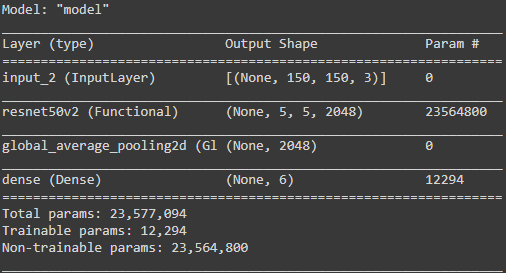
\includegraphics[scale=0.5]{gambar/model.png}
    % Keterangan gambar yang diinputkan
    \caption{Arsitektur Model}
    % Label referensi dari gambar yang diinputkan
    \label{fig:model}
  \end{figure}
  
  Untuk pembuatan model \textit{Machine Learning} kami menggunakan arsitektur ResNet-50.
  
  \subsection{\textit{Deployment} di \textit{Cloud}}
    
    \subsubsection{Cloud API}

    Sejatinya aplikasi \textbf{The Batik} yang terdapat di device Android tidak memiliki kapabilitas untuk melakukan identifikasi jenis batik melalui gambar yang diterima, melainkan menyerahkan tugas identifikasinya di Cloud.
    Untuk proyek ini digunakan layanan Google App Engine dari Google Cloud Platform untuk menjalankan program identifikasi gambar yang memanfaatkan model machine learning yang sudah dibuat lalu mengirimkan hasil prediksi jenis motif batik Kembali ke apikasi \textbf{The Batik} yang mengirimkan gambar tersebut.

    \subsubsection{Web Framework}

    Web Framework yang digunakan untuk aplikasi The Batik ini menggunakan FLASK yang menggunakan Bahasa pemrograman Python. Dalam program python yang di-\textit{deploy} dengan \textit{Web Framework} ini ke \textit{Cloud} terdapat beberapa fungsi yang digunakan untuk keberlangsungan prediksi motif batik yang dikirim oleh aplikasi Android--\textbf{The Batik}-- yang akan dijelaskan di subbab berikut.
    
    \subsubsection{REST API Routing}
    
    Agar program python yang di\textit{deploy} di \textit{cloud} dapat menerima kiriman gambar dari aplikasi Android, di dalam program python disediakan \textit{route} yang menggunakan REST API.
    Dalam kasus ini hanya memanfaatkan protocol POST dari REST API.
    Untuk membuat route bagi aplikasi \textbf{The Batik} dalam mengirimkan gambar, disediakan \textit{route} dengan alamat belakang \textbf{"/predict/full"}.
    Selain \textit{route} untuk prediksi, disediakan juga \textit{default route} untuk keperluan debugging jika proses \textit{deployment} tidak berhasil.

    \subsubsection{Load Keras Model}
    \label{loadKeras}
    Model \textit{Machine Learning} yang sudah dibuat perlu untuk dimuat terlebih dahulu sebelum bisa digunakan untuk memprediksi gambar yang diterima.
    Untuk memuat model, digunakan fungsi \lstinline{keras.models.load_model()} yang disediakan di dalam pustaka \textbf{Tensorflow} untuk python.
    Setelah dimuat, model bisa digunakan untuk memprediksi gambar yang diterima menggunakan fungsi \lstinline{model.predict}.
    Tetapi sebelum gambar bisa diprediksi, gambar perlu dilakukan \textit{preprocessing} terlebih dahulu.

    \subsubsection{\textit{Image Preprocessing}}

    Seperti dijelaskan di bagian Load Keras Model \nameref{loadKeras}, gambar perlu dilakukan \textit{preprocess} untuk keperluan pengiriman gambar melewati REST API dan memenuhi syarat format gambar yang diinginkan oleh model \textit{Machine Learning} yang sudah dibuat.
    Berikut ini prosesnya:

      \begin{enumerate}[nolistsep]

        \item Mendekode gambar dalam format base64.
        Gambar yang diterima dari request REST API berada dalam format encode base64.
        Menggunakan library base64, gambar dapat di decode dan akan menghasilkan output berupa byte yang lalu dibaca menggunakan fungsi imread dari pustaka imageio agar dirubah kedalam bentuk format gambar OpenCV.

        \item Mengubah gambar ke format sesuai model ML.
        Model ML yang digunakan memerlukan format gambar yang di susun menjadi 1 tensor dengan dimensi 150x150.
        Menggunakan library OpenCV untuk python, dapat dilakukan pemformatan ulang untuk gambar yang sudah di-decode agar dapat memenuhi syarat dari model. 
        Memprediksi motif Gambar dengan Model yang dimuat.
        Gambar yang sudah dipreprocess sesuai dengan kebutuhan model dapat di prediksi langung menggunakan fungsi model.predict() dengan menginputkan gambar ke dalam parameternya. Output yang diberikan dari hasil prediksi meliputi persenan kemungkinan dari tiap batik yang tersedia di di training dataset. 
        Hasil prediksi ini lah yang lalu dikirim balik sebagai response ke aplikasi The Batik.

      \end{enumerate}
    
    \subsection{Men\textit{deploy} Web Framework ke Google App Engine}
    
    Web Framework yang sudah lengkap perlu di upload ke Google Cloud Platform lengkap dengan keperluan lainnya seperti file model ML, file runtime, dan tambahan-tambahan lainnya.
    Sebelumnya, kelompok \textit{Capstone Project} sudah membuat akun Google Cloud Platform dan membuat project untuk pen\textit{deployan} web frameworknya.
    Kelengkapan Web Framework tadi di upload ke Google Shell sebelum di deploy ke App Engine.